\subsubsection*{\S 设计题}
\setcounter{problemname}{0}

\begin{problem}[2021]
分析下图界面,指出其中5处不合理的地方,并指出其违反的2条启发式设计规则,以及该规则的具体内容。请对该界面进行修改,并给出修改后的界面草图。
\begin{figure}[H]
    \vspace{-0.5em}
	\centering
	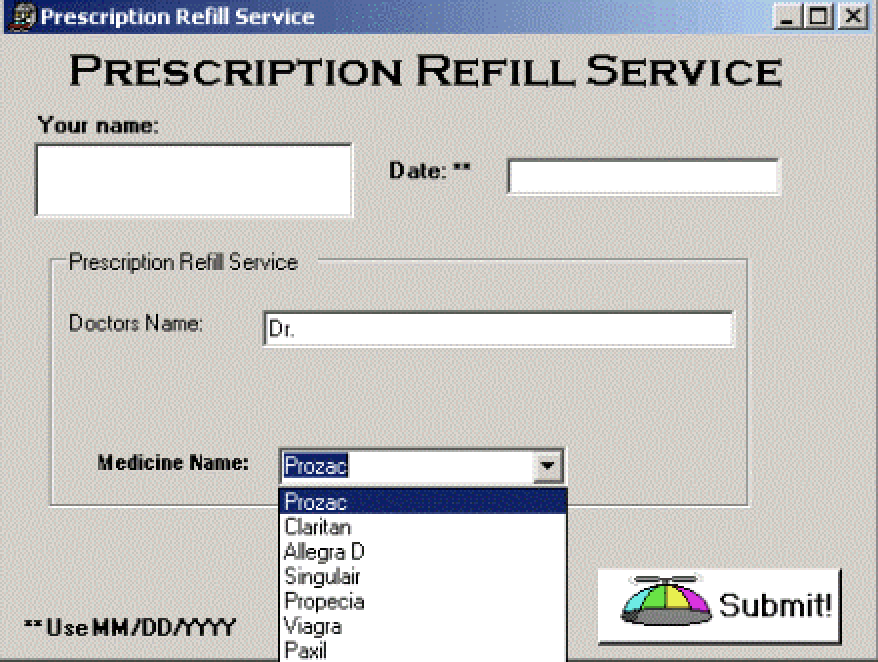
\includegraphics[width=0.5\textwidth]{1.png}
    \vspace{-1em}
\end{figure}
\end{problem}

\begin{solution}
不合理的地方:
\begin{enumerate}[label=\arabic*.]
    \item 日期不应当让用户输入:避免出错
    \item 应当使用用户听得懂得交互语言,而不是Use MM/DD/YYYY:系统与现实社会问题
    \item Submit的按钮左侧的图标没有意义:一致性和标准化
    \item 最上面的两个输入框没有对齐:标准化
    \item Your name、下拉框
\end{enumerate}

启发式设计规则:避免出错、一致化和标准化、灵活性和高效性
\end{solution}



\begin{problem}[2021]
可用性评估实验
\begin{enumerate}[label=\arabic*.]
    \item 目前市场上大多数移动电话都不是为老年人设计的。现在假设你需要为70岁以上的老年人设计一款移动电话,你会如何着手设计活动?需求分析阶段你将使用哪些技术?为什么?
    \item 需求分析之后,你制作了一些纸质原型,计划对他们的可用性进行评估,你将使用哪些评估方法?为什么?
    \item 假设你的设计方案被企业采纳,他们做出了一个完整的原型,并希望在开始批量生产前对其可用性进行评估。你将如何开展可用性评估?请简述评估过程。
\end{enumerate}
\end{problem}

\begin{solution}
\begin{enumerate}[label=\arabic*.]
    \item 
    \begin{enumerate}[label=(\arabic*)]
        \item 我会考虑到用户的年龄差异,提供对残缺部分的支持,更加注重容错和冗余。
        \item 技术:现场观察用户来获取同环境相关的问题。构建场景和人物角色,解决产品开发过程中出现的三个设计问题。头脑风暴等。
    \end{enumerate}
    \item 
    \begin{enumerate}[label=(\arabic*)]
        \item 快速评估、启发式评估。
        \item 在项目早期可以使用启发式评估,同时还可以结合快速评估来获取到用户的相关反馈信息。
    \end{enumerate}
    \item 
    \begin{enumerate}[label=(\arabic*)]
        \item 用户测试
        \item 选择被测试用户(三种)、开展预实验、使用DECIDE评估框架
    \end{enumerate}
\end{enumerate}
\end{solution}



\begin{problem}[2013、2022]
指出下面的对话框设计中存在的问题,并给出改进建议。
\begin{figure}[H]
    \vspace{-0.5em}
	\centering
	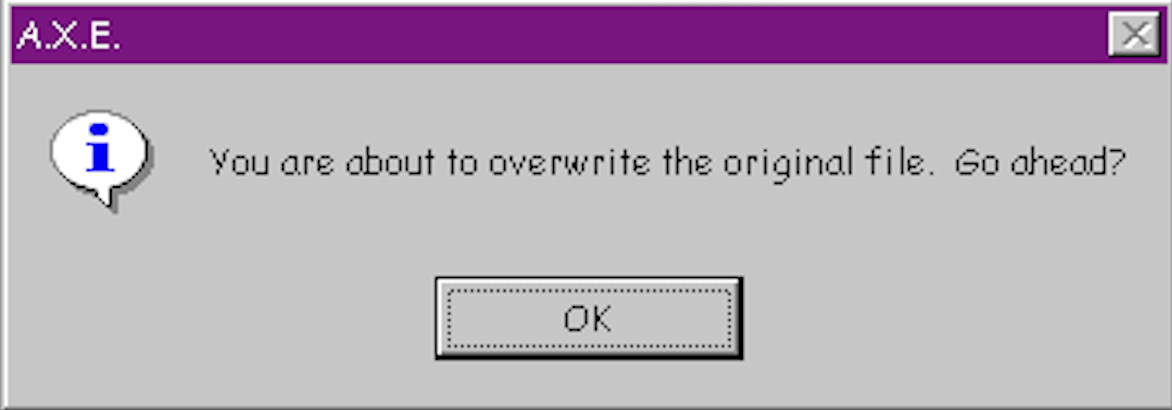
\includegraphics[width=0.5\textwidth]{20221.png}
    \vspace{-1em}
\end{figure}
\end{problem}

\begin{solution}
问题:对话框标题设计含义不明确,无法让用户一目了然对话框的目标;提示语过于冗长;只有ok的按钮,没有放弃的按钮,不便于用户中途改变主意。

建议:标题改为``Hint;提示语改为``Overwrite the original file?";按钮修改为 ``OK" , ``Cancel"。
\end{solution}




\begin{problem}[2022]
人物角色是交互设计中非常重要的一项技术,能够帮助设计团队做很多设计决策。如下是某团队为某项目构造的人物角色的例子,请分析其中存在的问题,并说明什么是人物角色,以及在构建人物角色时需要注意哪些问题。
\begin{figure}[H]
    \vspace{-0.5em}
	\centering
	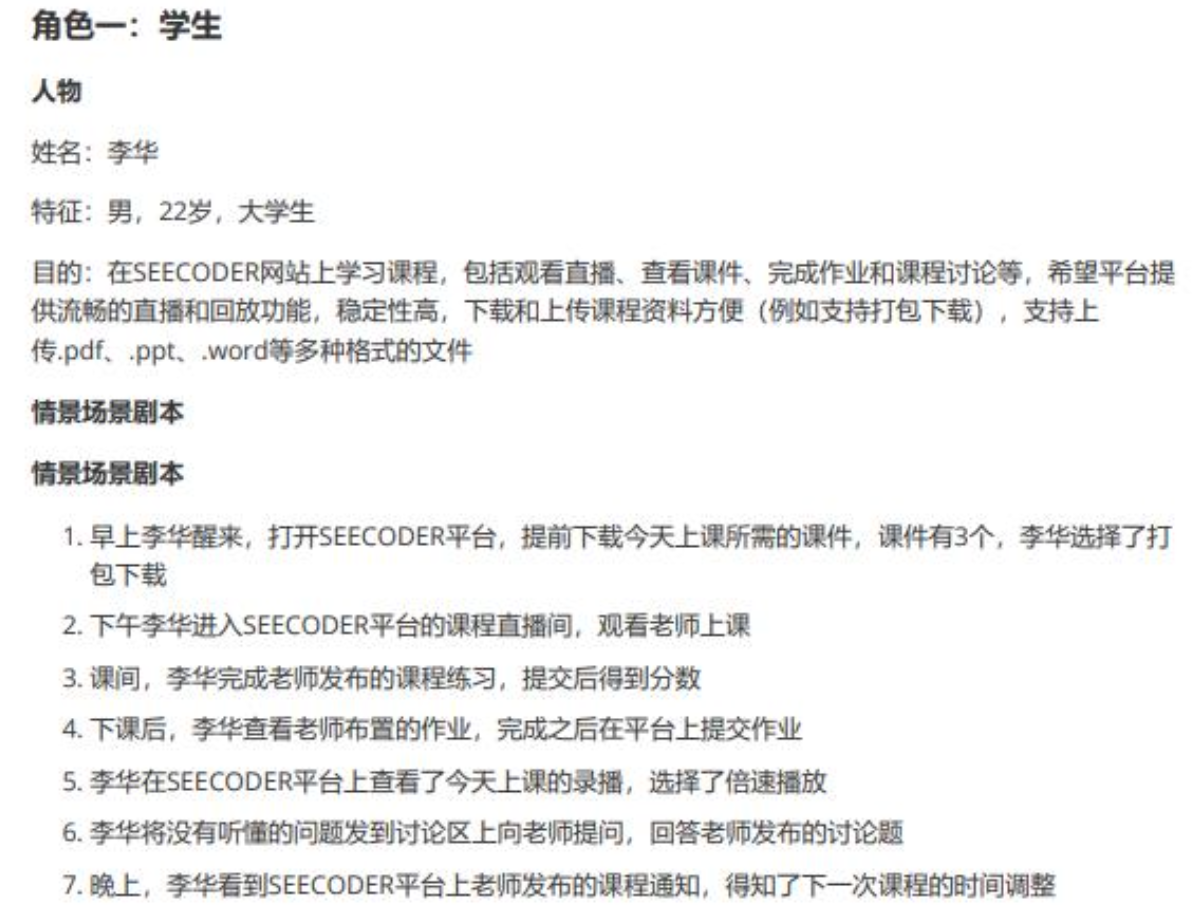
\includegraphics[width=0.7\textwidth]{20222.png}
    \vspace{-1em}
\end{figure}
\end{problem}

\begin{solution}
问题:
\begin{enumerate}[label=\arabic*.]
    \item 人物信息构造不完整(没有照片);
    \item 目标不对,目标不是功能(帮助他更好的完成课程学习);
    \item 场景剧本有问题(不能写成使用手册,应该描述需求,不要使用术语,要使用自然语言);
\end{enumerate}

人物角色是基于观察到的那些真实人的行为和动机,并且在整个设计过程中代表真实的人;是在人口统计学调查收集到的实际用户的行为数据的基础上形成的综合原型。

要注意那些与软件用户界面设计有关的角色特征;要关注使角色之间彼此相区别的特征;要留心焦点角色 (最常见、最典型的角色)。
\end{solution}




\begin{problem}[2013、2015、2022]
为下列每一种情况选择一个适当的评估方法。在每一种情况中确定:
\vspace{-0.8em}
\begin{multicols}{4}
    \begin{enumerate}[label=\arabic*.]
        \item 典型用户
        \item 应用的技术
        \item 代表性的测试任务
        \item 评价标准
    \end{enumerate}
\end{multicols}
\vspace{-1em}
\begin{enumerate}[label=\arabic*.,start=5]
    \item 实验过程(简要描述即可,不需要罗列详细测试步骤)
\end{enumerate}

具体情况包括:
\begin{enumerate}[label=\alph*.]
    \item 在电子制表软件包的设计初期阶段,你要测试哪种类型的图标最容易学习。
    \item 你有一个戏院订票系统的原型,潜在的戏迷应用它能减少在售票处前排队。
    \item 你已经设计和实现了一个新的游戏系统,在发布以前你想对其进行评估。
    \item 已经要求你开发一个存储和管理学生考试结果的系统。在实现和给出原型之前,你希望对两个不同的设计进行测试。
\end{enumerate}
\end{problem}

\begin{solution}
\begin{enumerate}[label=\alph*.]
    \item 
    \begin{enumerate}[label=\arabic*.]
        \item 评估方法:用户观察、专家访问
        \item 典型用户:一些商务人士,需要经常使用到电子制表软件
        \item 应用的技术:访谈(对专家),用户观察、问卷调查
        \item 代表性测试任务:询问专家主流电子制表软件说使用的图标;将不同类型的图标发给不同的用户,相同时间后考察用户学习情况
        \item 评价标准:就专家访问,统计不同专家的观点,推荐多的为优;就用户观察,比较用户学习情况,能记住85\%为好,70\%为普通,低于70\%为差
        \item 实验过程:准备已有的若干套图标,询问专家,听取建议,并做记录;选择$N$组用户,分别用$N$套不同的图片让他们学习,学习时间为10分钟,然后进行测试,考察学习情况
    \end{enumerate}
    \item 
    \begin{enumerate}[label=\arabic*.]
        \item 评估方法:用户测试
        \item 典型用户:戏迷
        \item 应用的技术:DECIDE模式
        \item 代表性测试任务:比较新订票系统和原有订票方式的效率
        \item 评价标准:新系统订票所有时间比原有订票方式快15\%为好,10\%-15\%为普通,小于10\%为差
        \item 实验过程:让两组用户分别用新旧两种方式进行订票,记录时间,统计分析
    \end{enumerate}
    \item 
    \begin{enumerate}[label=\arabic*.]
        \item 评估方法:用户测试、用户观察
        \item 典型用户:游戏爱好者
        \item 应用的技术:边说边做、DECIDE模式
        \item 代表性测试任务:新游戏系统的可用性和用户体验情况
        \item 评价标准:对于界面,用户满意度>85\%为优,70\%-85\%普通,70\%以下为差;对于游戏情节设置:响应时间为优
        \item 实验过程:安排用户学习体验游戏系统,可在过程中有道用户说出自己想法,并进行记录。之后发放问卷调查用户体验,统计数据,分析
    \end{enumerate}
    \item 
    \begin{enumerate}[label=\arabic*.]
        \item 评估方法:专家访问
        \item 典型用户:教务人员老师
        \item 应用的技术:问卷调查、访谈
        \item 代表性测试任务:了解用户对于两个设计方案的看法,并进行比较
        \item 评价标准:在不同的方面分别进行比较,用户满意度高的优
        \item 实验过程:安排用户在一个安静的环境中,将两个设计方案向用户描述,听去用户建议,再发放问卷,对不同方面进行调查,统计数据、分析
    \end{enumerate}
\end{enumerate}
\end{solution}



\begin{problem}[2012]
1. 用适当的标题将下列功能分组,假设所选择标题将作为一个菜单驱动的字处理系统的基础,功能将出现在对应的标题之下。菜单标题的数目可以自行控制。如果愿意,也可以稍微更改功能的叫法。
    
save, save us, new, delete, open mail, send mail, quit, undo, table, glossary(词汇表、术语表), preferences, character style, format paragraph, lay out document, position on page, plain text, bold text, italic text, underline, open file, close file, open copy of file, increase point size, decrease point size, change font, add footnote, cut, copy, paste, clear, repaginate(重新分页), add page break, insert graphic, insert index entry, print, print preview, page setup, view page, find word, change word, go to, go back, check spelling, view index, see table of contents, count words, renumber pages, repeat edit, show alternative document, help

2. 考虑下面的问题:可以把功能分在三个菜单上,使每一个菜单都有很多功能;或者分在八个菜单上,使每一个菜单的功能比较少。哪一种做法比较容易使用?为什么?设计一个实验来测试你的答案。
\end{problem}

\begin{solution}
\begin{enumerate}[label=\arabic*.]
    \item File: new, save, save as, quit, undo position on page, open file, close file, preferences, open copy of file, print, print preview
    \item Edit: deletecut, copy, paste, clear, go to, count words,  find word, change word, repeat edit,  go back
    \item View: underline, repaginate, page setup, view page, see table of contents, count words, renumber pages, show alternative document
    \item Insert: Insert graphic, insert index entry, add footnote, table, glossary, help
    \item Format: plain text, bold text, italic text, increase point size, decrease point size, change font, format paragraph, character style
\end{enumerate}

如果把功能分在三个菜单上,每个菜单都有很多功能,用户可能会感到一开始比较复杂,但一旦他们习惯了,使用起来可能会更高效。另一方面,分在八个菜单上,每个菜单的功能比较少,可能更容易让用户一开始就找到他们需要的功能,但可能会导致在不同菜单之间频繁切换。

为了测试哪一种做法更容易使用,可以进行一个用户体验实验。招募一组代表用户群体的参与者,分别让他们使用两种设计进行一系列任务。观察和记录以下方面的数据:任务完成时间、错误率、用户满意度、学习曲线、菜单切换频率。

\end{solution}



\begin{problem}[2012]
为一个帮助儿童学习数学运算(如 10 以内加减法)的软件系统选择恰当的交互范型。该软件的核心可用性准则有哪些?应如何度量?
\end{problem}

\begin{solution}
范型:自然语言交互。

准则和度量:
\vspace{-0.8em}
\begin{multicols}{2}
    \begin{enumerate}[label=\arabic*.]
        \item 易学性:用户达到某一熟练程度所需的时间
        \item 易记性:用户完成特定任务后解释
        \item 少出错:出错的频率
        \item 用户满意度:在用户使用后进行调查
    \end{enumerate}
\end{multicols}
\vspace{-1em}
\end{solution}



\begin{problem}[2015]
如下是一个系统的界面。初始时所有输入框不可输入,点击Edit时Point可修改;点击Add New时,所有输入框内容清空;点击Save时保存所有修改;点击Cancel时,取消所做的内容变更。举出三个界面设计不当之处,并简要分析;举出违反的三条启发式规则,并简要说明。

\begin{figure}[H]
    \vspace{-0.5em}
    \centering
    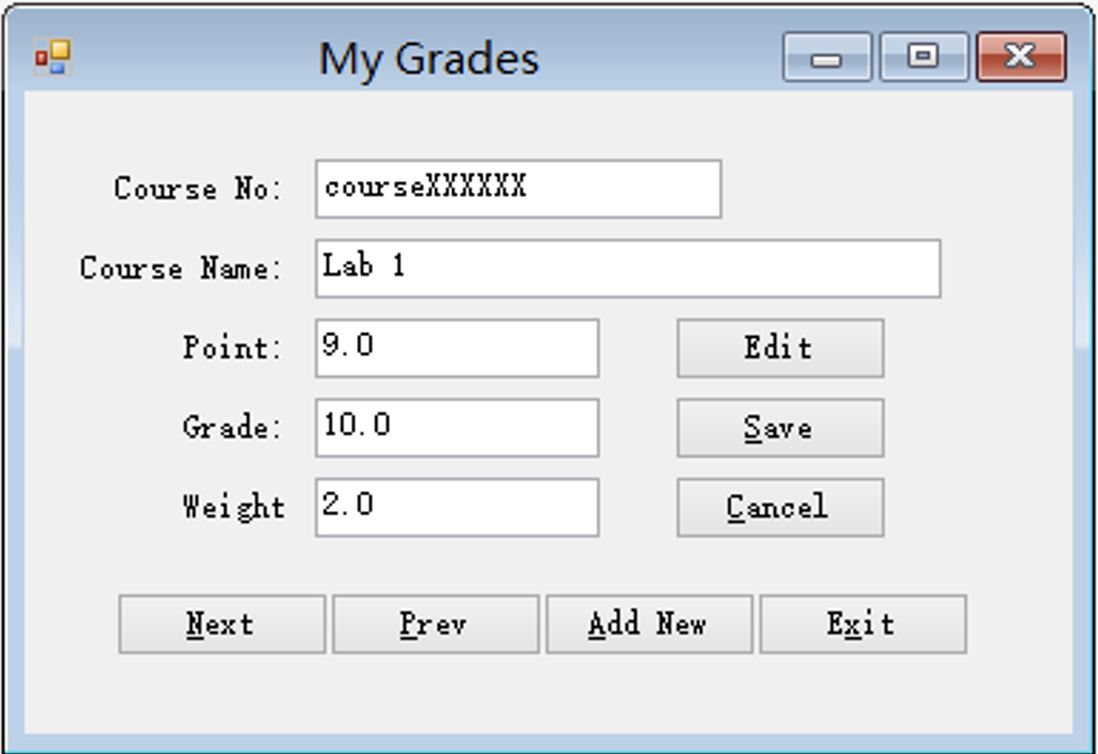
\includegraphics[width=0.5\textwidth]{2015JavaSwing.png}
    \vspace{-1em}
\end{figure}
\end{problem}

\begin{solution}
设计不当之处:Next、Prev;不可输入应当使得输入栏灰色;Add New点击后清空数据;缺少必要的说明文档。

违反的启发式规则:一致化和标准化;避免出错;灵活性和高效性;文档和帮助。
\end{solution}



\begin{problem}[2012]
在使用 MS Word 软件画图时,选择“自选图形 $\rightarrow$ 其他自选图形”时,屏幕会弹出如下图所示安装错误的提示框。点击取消后,该提示框仍会反复出现,直至使用任务管理器将winword进程关闭。请使用Nielsen的十条启发式规则解释该设计违背了哪一条设计原则,应该如何改进。

\begin{figure}[H]
    \vspace{-0.5em}
    \centering
    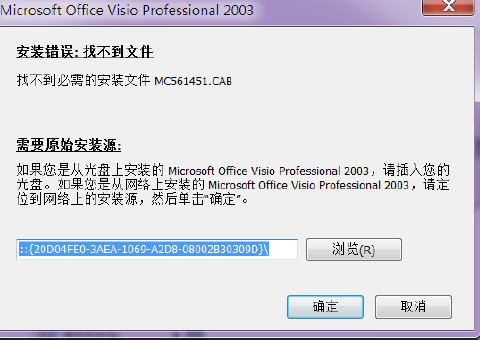
\includegraphics[width=0.65\textwidth]{2012word.png}
    \vspace{-1em}
\end{figure}
\end{problem}

\begin{solution}
用户享有控制权和自主权。让用户能够退出异常状态。
\end{solution}



\begin{problem}[2012]
找出下图调查问卷片段中存在的主要问题。

\begin{figure}[H]
    \vspace{-0.5em}
    \centering
    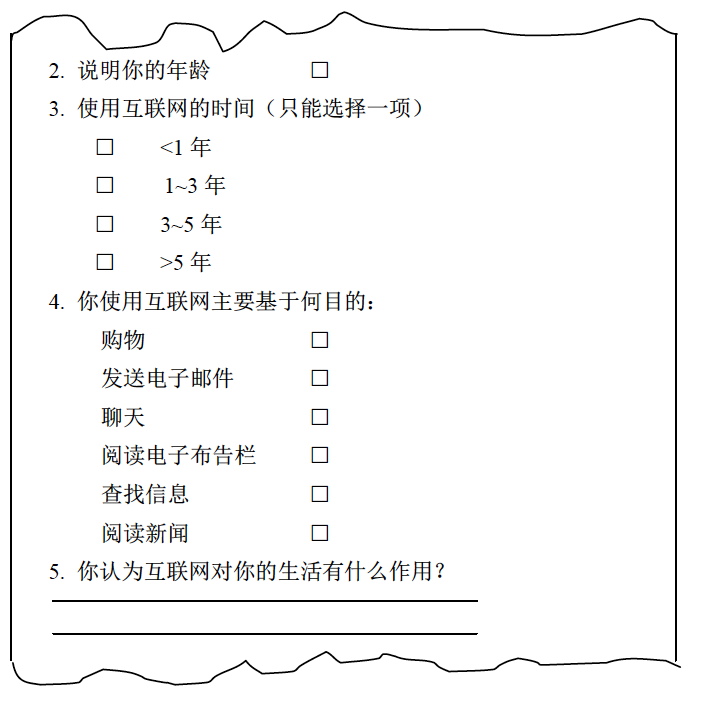
\includegraphics[width=0.55\textwidth]{2012问卷.png}
    \vspace{-1em}
\end{figure}
\end{problem}

\begin{solution}
说明你的年龄不够明确:没有指出格式等信息;应当提供“没有使用互联网”的选项;说明如何完成问卷。
\end{solution}



\begin{problem}[2015]
有一个摄氏/华氏温度转换工具,用户选择转换模式后,在第一个文本框内输入待转换的温度,按回车即在第二个文本框内显示转换后的温度。初始时,用户的手在键盘上。用KLM模型分析用户完成将27.3摄氏度转换成华氏度所需的操作时间。

\begin{figure}[H]
    \vspace{-0.5em}
    \centering
    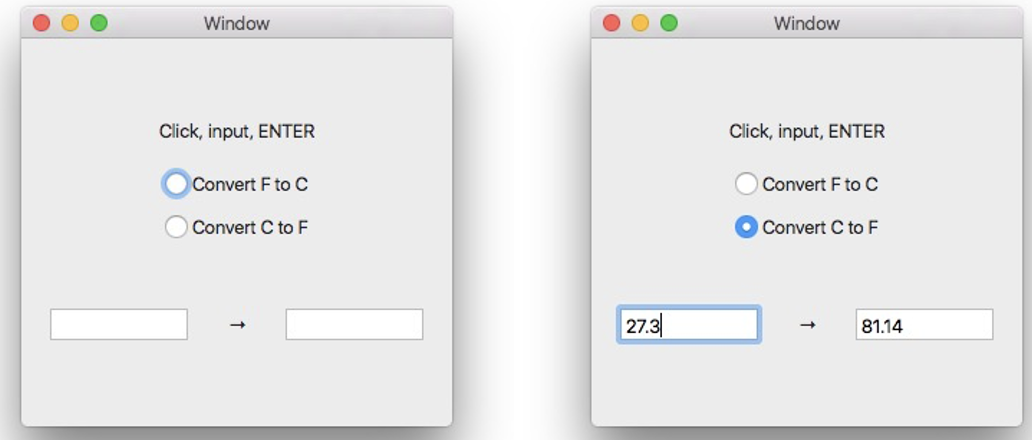
\includegraphics[width=0.75\textwidth]{2015KLM.png}
    \vspace{-1em}
\end{figure}
\end{problem}
